\documentclass[12pt,fleqn,handout]{beamer}


\xdefinecolor{lavendar}{rgb}{0.8,0.6,1}
\xdefinecolor{olive}{cmyk}{0.64,0,0.95,0.4}
%\xdefinecolor{olive}{cmyk}{1,0,0,0}
\xdefinecolor{mag}{cmyk}{0.1,1,0,0.2}
\xdefinecolor{lblue}{rgb}{0,0,1.5}
\xdefinecolor{lred}{rgb}{1,0,0}
\xdefinecolor{mine}{cmyk}{1,0,0.2,0}
\xdefinecolor{bluel}{cmyk}{0.1,0,0.9,0.4}

\usepackage{amsmath,amssymb,dsfont,mathrsfs}
\usepackage{tikz,pgflibraryplotmarks}
\usepackage{multimedia}
\usepackage{wasysym}
\usepackage{rotating}
\usepackage{algorithm,algorithmic}
\usepackage{graphicx} % more modern
\usepackage{subfigure}
\usepackage{booktabs}

\usepackage{pgfplots}
\usepackage{verbatim}

\usepackage{setspace}
\newlength\iwidth
\newlength\iheight

\newcommand\makebeamertitle{\frame{\maketitle}}%
\graphicspath{{./images/}}
\setbeamertemplate{navigation symbols}{}
\addtobeamertemplate{navigation symbols}{}{%
    \usebeamerfont{footline}%
    \usebeamercolor[fg]{footline}%
	\insertshorttitle
    \;--
    \insertframenumber
}

\newcommand{\sectionstart}{
	\only<beamer>{
 	\begin{frame}% (fold)
 		\begin{centering}\Huge \insertsection \par\end{centering}
 	\end{frame}% frame the_application (end)
	}
 }


% make bibliography entries smaller
\usepackage{natbib}
\setbeamertemplate{bibliography item}{[\theenumiv]}
\renewcommand\bibfont{\scriptsize}
\setbeamertemplate{frametitle continuation}[from second]
\newcommand{\tcr}{\textcolor{red}}
\newcommand{\tcrd}{\textcolor{red}}
\newcommand{\tcb}{\textcolor{bluel}}
\newcommand{\tcm}{\textcolor{mag}}
\newcommand{\tcg}{\textcolor{olive}}

\newcommand{\R}{\mathbb{R}}
\newcommand{\C}{\mathbb{C}}

% bold lower-case for vectors
\newcommand{\bfa}{{\bf a}}
\newcommand{\bfb}{{\bf b}}
\newcommand{\bfc}{{\bf c}}
\newcommand{\bfs}{{\bf s}}
\newcommand{\bfm}{{\bf m}}
\newcommand{\bfd}{{\bf d}}
\newcommand{\bfe}{{\bf e}}
\newcommand{\bfu}{{\bf u}}
\newcommand{\bfy}{{\bf y}}
\newcommand{\bfx}{{\bf x}}
\newcommand{\bfh}{{\bf h}}
\newcommand{\bfw}{{\bf w}}
\newcommand{\bfv}{{\bf v}}
\newcommand{\bfr}{{\bf r}}
\newcommand{\bfz}{{\bf z}}
\newcommand{\bfp}{{\bf p}}


% bold upper-case for linear operators
\newcommand{\bfA}{{\bf A}}
\newcommand{\bfB}{{\bf B}}
\newcommand{\bfZ}{{\bf Z}}
\newcommand{\bfM}{{\bf M}}
\newcommand{\bfC}{{\bf C}}
\newcommand{\bfD}{{\bf D}}
\newcommand{\bfQ}{{\bf Q}}
\newcommand{\bfJ}{{\bf J}}
\newcommand{\bfG}{{\bf G}}
\newcommand{\bfI}{{\bf I}}
\newcommand{\bfP}{{\bf P}}
\newcommand{\bfK}{{\bf K}}
\newcommand{\bfY}{{\bf Y}}
\newcommand{\bfW}{{\bf W}}
\newcommand{\bfR}{{\bf R}}
\newcommand{\bfL}{{\bf L}}
\newcommand{\bfF}{{\bf F}}
\newcommand{\bfT}{{\bf T}}
\newcommand{\bfS}{{\bf S}}
\newcommand{\bfX}{{\bf X}}
\newcommand{\bfU}{{\bf U}}
\newcommand{\bfV}{{\bf V}}
\newcommand{\bfH}{{\bf H}}


\newcommand{\calF}{\mathcal{F}}



\newcommand{\hf}{{\frac 12}}
\newcommand{\bftheta}{{\boldsymbol \theta}}
\newcommand{\bfxi}{{\boldsymbol \xi}}

\newcommand{\bfLambda}{{\boldsymbol \Lambda}}
\newcommand{\bfSigma}{{\boldsymbol \Sigma}}
\newcommand{\bfepsilon}{{\boldsymbol \epsilon}}

\newcommand{\E}{\vec E}
\newcommand{\B}{\vec B}

\newcommand{\vu}{  {\vec {\bf u}}}

\newcommand{\grad}{  {\vec {\bf \nabla}}}

\newcommand{\lfrownie}{\textcolor{red}{\large{\frownie}}}
\newcommand{\lsmiley}{\textcolor{green}{\large{\smiley}}}

\newcommand{\curl}{\ensuremath{\nabla\times\,}}
\renewcommand{\div}{\nabla\cdot\,}
\newcommand{\divh}{\nabla_h\cdot\,}
\renewcommand{\grad}{\ensuremath{\nabla}}

\DeclareMathOperator*{\argmin}{arg\,min}

\title{Parametric Models}
\subtitle{Numerical Methods for Deep Learning}
\date{}
\begin{document}

\makebeamertitle

\section{Parametric Models} % (fold)
\label{sec:parametric_models}
\begin{frame}[fragile]\frametitle{Motivation}

Recall single layer
$$
	\bfZ = \sigma(\bfK\bfY + \bfb),
$$
where $\bfY \in \R^{n_f\times n}, \bfK \in \R^{m \times n_f}, \bfb\in\R^m$, and $\sigma$ element-wise activation. 

\bigskip
\pause

We saw that $m \gg n_f$ needed to fit training data. 

Conservative example: Consider MNIST ($n_f = 28^2$) and use $m=n_f$ $\leadsto 614,656$ unknowns for a single layer. \pause Famous quote:

\begin{quote}
	With four parameters I can fit an elephant, and with five I can make him wiggle his trunk.
\end{quote}

\bigskip
\pause

Possible remedies:
\begin{itemize}
	\item \textbf{Regularization:} penalize $\bfK$ 
	\item \textbf{Parametric model:} $\bfK(\bftheta)$ where $\bftheta\in\R^p$ with $p\ll m\cdot n_f$.
\end{itemize}
\end{frame}


\begin{frame}\frametitle{Some Simple Parametric Models}
	
	\begin{itemize}
		\item Diagonal scaling:
		$$
			\bfK(\bftheta) = {\rm diag}(\bftheta) \in \R^{n_f\times n_f}
		$$
		Advantage: preserves size and structure of data.
		\pause
		\item Antisymmetric kernel
		$$
			\bfK(\bftheta) = \left(
				\begin{array}{rrr}
					0 & \bftheta_1 & \bftheta_2 \\
					-\bftheta_1 & 0 & \bftheta_3 \\
					-\bftheta_2 & -\bftheta_3 & 0
				\end{array}
			\right)
		$$
		Advantage?: ${\rm real}(\lambda_i(\bfK(\bftheta))) = 0$. 
		\pause
		\item $M$-matrix
		$$
		\bfK(\bftheta) = \left(
				\begin{array}{rrr}
					\bftheta_1+\bftheta_2 & -\bftheta_1 & -\bftheta_2 \\
					-\bftheta_3 & \bftheta_3 + \bftheta_4 & -\bftheta_4 \\
					-\bftheta_5 & -\bftheta_6 & \bftheta_5+\bftheta_6
				\end{array}
			\right)
			\quad \bftheta \geq 0
		$$
		Advantage: like differential operator
	\end{itemize}
\end{frame}

\begin{frame}
	\frametitle{Differentiating Parametric Models}
	Need derivatives of model to optimize $\bftheta$ in
	$$
		E(\bfW \sigma(\bfK(\bftheta)\bfY+\bfb),\bfC) 
	$$
	(we can re-use previous derivatives and use chain rule)
	
	\bigskip
	\pause
	
	Note that all previous models are linear in the following sense
	$$
		\bfK(\bftheta) = {\rm mat}(\bfQ\, \bftheta)
	$$
	
	\bigskip
	\pause
	
	Therefore, matrix-vector products with the Jacobian simply are
	$$
		\bfJ_\bftheta (\bfK(\bftheta)) \bfv  = {\rm mat}(\bfQ \ \bfv)\quad\text{ and }\quad
		\bfJ_\bftheta (\bfK(\bftheta))^\top \bfw  = \bfQ^\top \bfw
	$$
	where $\bfv \in \R^p$ and $\bfw \in \R^m$.
\end{frame}

\begin{frame}\frametitle{Example: Derivative of M-matrix}
	$$
	\bfK(\bftheta) = \left(
			\begin{array}{rrr}
				\bftheta_1+\bftheta_2 & -\bftheta_1 & -\bftheta_2 \\
				-\bftheta_3 & \bftheta_3 + \bftheta_4 & -\bftheta_4 \\
				-\bftheta_5 & -\bftheta_6 & \bftheta_5+\bftheta_6
			\end{array}
		\right)
		\quad \bftheta \geq 0
	$$
	\pause
	verify that this can be written as $K(\bftheta) = {\rm mat}(\bfQ \, \bftheta)$ where
	$$
		\bfQ = \left(
			\begin{array}{rrrrrr}
				1 & 1 & 0 & 0 & 0 & 0 \\
				0 & 0 & -1& 0 & 0 & 0 \\
				0 & 0 & 0 & 0 &-1 & 0 \\
				-1& 0 & 0 & 0 & 0 & 0 \\
				0 & 0 & 1 & 1 & 0 & 0 \\
				0 & 0 & 0 & 0 & 0 &-1 \\
				0 &-1 & 0 & 0 & 0 & 0 \\
				0 & 0 & 0 & -1& 0 & 0 \\
				0 & 0 & 0 & 0 & 1 & 1
			\end{array}
		\right) \in \R^{9\times 6}
	$$
	\begin{center}
		Note: not efficient to construct $\bfQ$ when $p$ large but helpful when computing derivatives
	\end{center}
\end{frame}

\begin{frame}\frametitle{Convolutional Neural Networks~\cite{LeCun1990}}
	\begin{center}
		\begin{tikzpicture}
			\node at (-3,0){
\includegraphics[width=4cm]{E13Conv2D-Y}};
			\node at (0.3,0){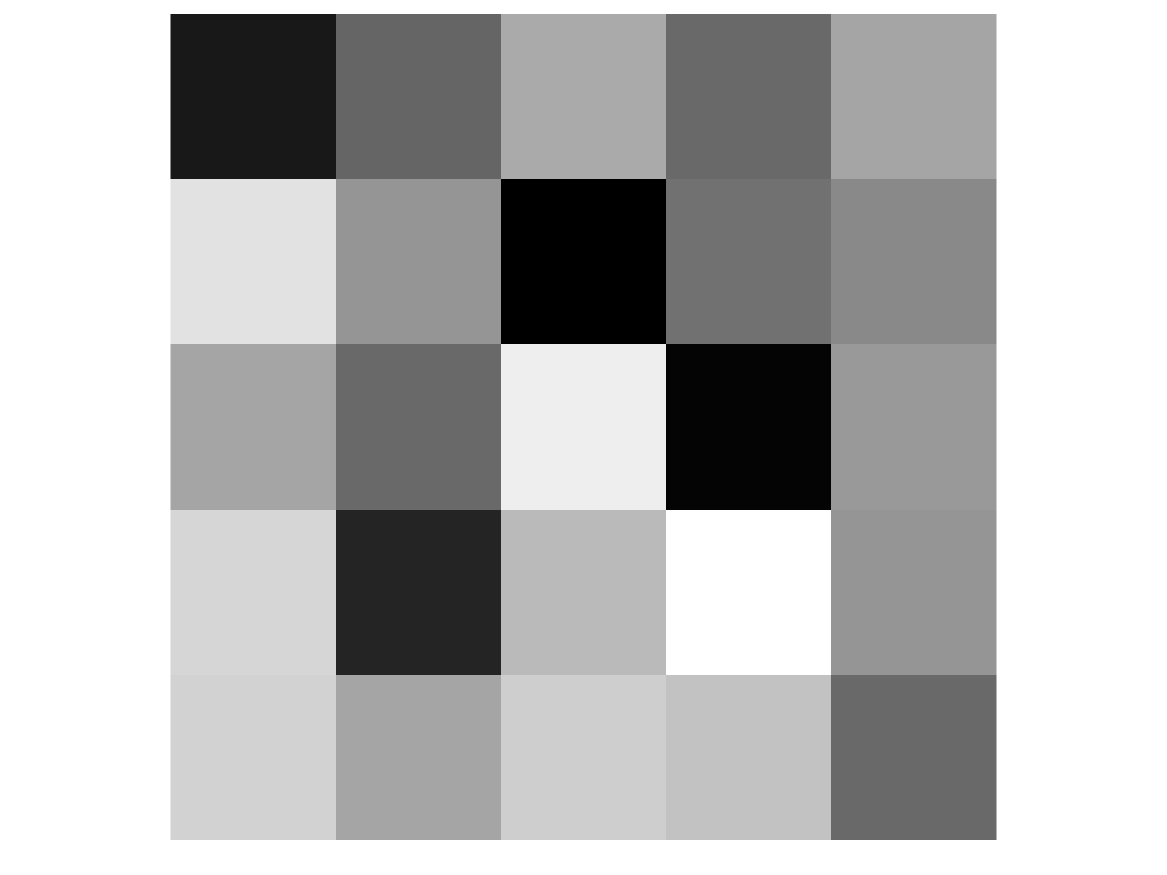
\includegraphics[width=1cm]{E13Conv2D-theta}};
			\node at (3,0){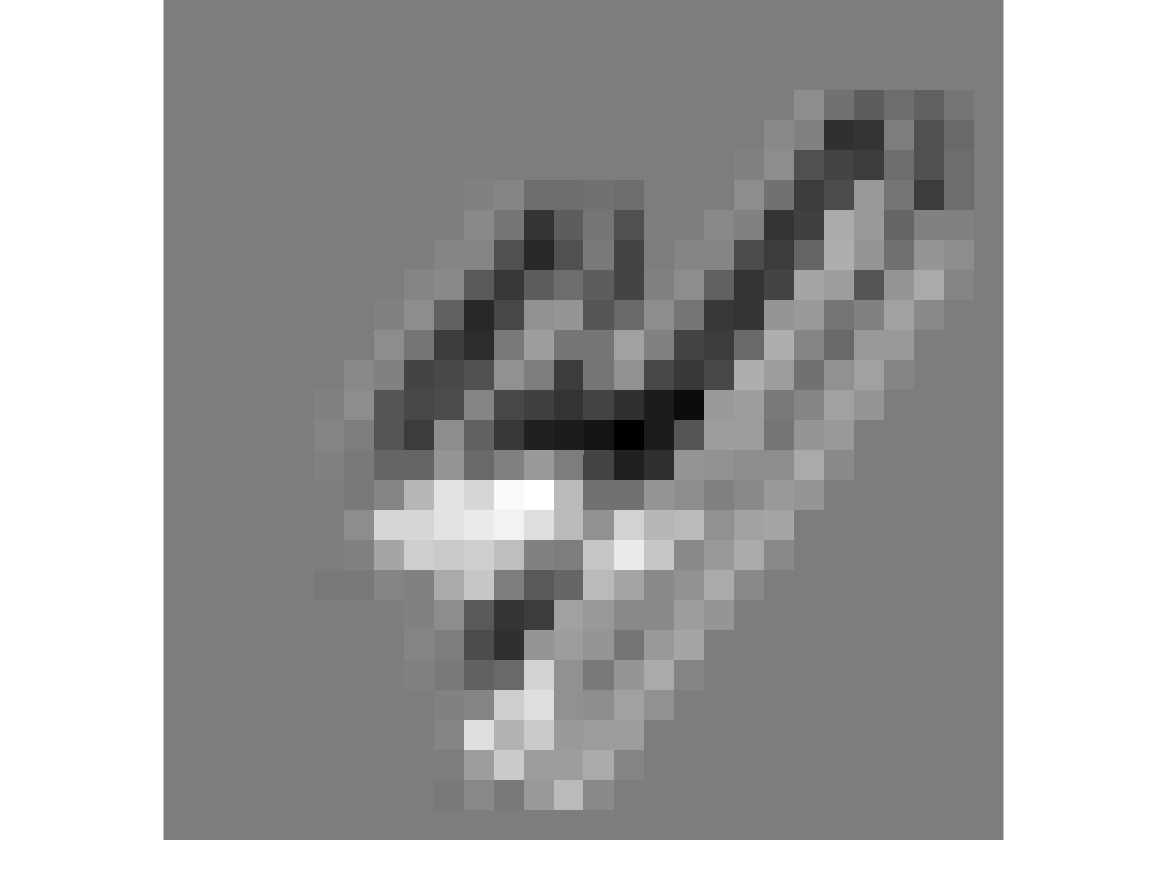
\includegraphics[width=4cm]{E13Conv2D-Z}};
			\node at (-2.3,+2.1){\small $\bfy \in \R^{28\times28}$ input features};
			\node at (0,-2.2){\small \textcolor{red}{$\bftheta\in\R^{5\times 5}$ convolution kernel}};
			\node at (+2.4,+2.1){\small$\bfz\in\R^{28\times 28}$ output features};
			\draw[->,red,thick] (0.3,-.5 ) edge (0.3,-2);
		\end{tikzpicture}
	\end{center}
	\begin{itemize}
		\item useful for speech, images, videos, \ldots
		\item efficient parameterization, efficient codes (GPUs, \ldots)
		\item later: CNNs as parametric model and PDEs, simple code
		\item see \texttt{E13Conv2D.m}
	\end{itemize}

\end{frame}

\begin{frame}\frametitle{Convolutions in 1D}
	Let $y, z, \theta:\R \to \R$, $z : \R\to\R$ be continuous functions then
	\begin{equation*}
		z(x) = (\theta * y)(x) = \int_{-\infty}^\infty \theta(x-t) y(t) dt.
	\end{equation*}
	Assume $\theta(x) \neq 0$ only in interval $[-a,a]$ (compact support).
	
	\bigskip
	\pause
	
	A few properties
	\begin{itemize}
	\item $ \theta * y = {\cal F}^{-1}(({\cal F} \theta) ({\cal F} y))$, ${\cal F}$ is Fourier transform
	\item $ \theta * y =  y * \theta$ 
	\end{itemize}
	
	
\end{frame}	

\begin{frame}\frametitle{Discrete Convolutions in 1D}
	Let $\bftheta \in\R^{2k+1}$ be stencil, $\bfy \in \R^{n_f}$ grid function
\begin{equation*}
		\bfz_i = (\bftheta * \bfy)_i = \sum_{j=-k}^k \bftheta_{j} \bfy_{i-1}.
	\end{equation*}
	
	\bigskip
	\pause

	 Example: Discretize $\bftheta \in \R^3$ (non-zeros only), $\bfy,\bfz \in \R^4$ on regular grid
	 \begin{align*}
	 	\bfz_1 & = \bftheta_3 \textcolor{red}{\bfw_1} + \bftheta_2 \bfx_1 + \bftheta_1 \bfx_2 \\
	 	\bfz_2 & = \bftheta_3 \bfx_1 + \bftheta_2 \bfx_2 + \bftheta_1 \bfx_3 \\
	 	\bfz_3 & = \bftheta_3 \bfx_2 + \bftheta_2 \bfx_3 + \bftheta_1 \bfx_4 \\
	 	\bfz_4 & = \bftheta_3 \bfx_3 + \bftheta_2 \bfx_4 + \bftheta_1 \textcolor{red}{\bfw_2}
	 \end{align*}
	 where $\textcolor{red}{\bfw_1, \bfw_2}$ are used to implement different boundary conditions (right choice? depends \ldots).
\end{frame}

\begin{frame}
	\frametitle{Structured Matrices - 1}
	$$
		\left( 
		\begin{array}{r}
			\bfz_1\\
			\bfz_2\\
			\bfz_3\\
			\bfz_4
		\end{array}
		\right)
		=
		\left( 
		\begin{array}{rrrrrrr}
			\bftheta_3 & \bftheta_2 & \bftheta_1 &          &          &           \\
			         & \bftheta_3 & \bftheta_2 & \bftheta_1 &          &           \\
			         &          & \bftheta_3 & \bftheta_2 & \bftheta_1 &           \\
			         &          &          & \bftheta_3 & \bftheta_2 & \bftheta_1 \\
		\end{array}
		\right)
		\left( 
		\begin{array}{r}
			\bfw_1\\
			\bfx_1\\
			\bfx_2\\
			\bfx_3\\
			\bfx_4\\
			\bfw_2
		\end{array}
		\right)
	$$
	Different boundary conditions lead to different structures
	\pause
	\begin{itemize}
		\item Zero boundary conditions: $\bfw_1 = \bfw_2 = 0$
	$$
		\left( 
		\begin{array}{r}
			\bfz_1\\
			\bfz_2\\
			\bfz_3\\
			\bfz_4
		\end{array}
		\right)
		=
		\left( 
		\begin{array}{rrrrr}
			\bftheta_2 & \bftheta_1 &          &           \\
			\bftheta_3 & \bftheta_2 & \bftheta_1 &           \\
			         & \bftheta_3 & \bftheta_2 & \bftheta_1  \\
			         &          & \bftheta_3 & \bftheta_2 \\
		\end{array}
		\right)
		\left( 
		\begin{array}{r}
			\bfx_1\\
			\bfx_2\\
			\bfx_3\\
			\bfx_4\\
		\end{array}
		\right)
	$$		
	This is a \emph{Toeplitz matrix} (constant along diagonals).
	\end{itemize}
\end{frame}

\begin{frame}
	\frametitle{Structured Matrices - 2}
	\begin{itemize}
		\item Periodic boundary conditions: $\bfw_1 = \bfx_4$ and $\bfw_2 = \bfx_1$
	$$
		\left( 
		\begin{array}{r}
			\bfz_1\\
			\bfz_2\\
			\bfz_3\\
			\bfz_4
		\end{array}
		\right)
		=
		\left( 
		\begin{array}{rrrr}
			        \bftheta_2 & \bftheta_1 &          & \bftheta_3  \\
			        \bftheta_3 & \bftheta_2 & \bftheta_1 &           \\
			                 & \bftheta_3 & \bftheta_2 & \bftheta_1  \\
			        \bftheta_1 &          & \bftheta_3 & \bftheta_2  \\
		\end{array}
		\right)
		\left( 
		\begin{array}{r}
			\bfx_1\\
			\bfx_2\\
			\bfx_3\\
			\bfx_4\\
		\end{array}
		\right)
	$$
	this is a \emph{circulant matrix} (each row/column is periodic shift of previous row/column)
	\end{itemize}
	\pause
	
	An attractive property of a circulant matrix is that we can efficiently compute its eigendecomposition
	$$
		\bfK(\bftheta) = \bfF^* {\rm diag}(\bflambda) \bfF
	$$ 
	where $\bfF$ is the discrete Fourier transform and the eigenvalues, $\bflambda \in {\mathbb{C}}^4$, can be computed using first column
	$$
		\bflambda =   \bfF( \bfK(\bftheta) \bfu_1) \quad \text{ where} \quad \bfu_1 = (1,0,0,0)^\top.
	$$ 	
\end{frame}

\begin{frame}\frametitle{Coding: 1D Convolution using FFTs}
	Let $\bftheta \in \R^3$ be some stencil and $n_f = m = 16$ 
\begin{enumerate}
	\item build a sparse matrix $\bfK$ for computing the convolution with periodic boundary conditions. 
	Hint: \texttt{spdiags}
	
	\item compute the eigenvalues of $\bfK$ using \texttt{eig(full(K))} and using $\texttt{fft}$ and first column of $\bfK$. Compare!
	
	\item verify that \texttt{norm(K*y - real(ifft(lam.*fft(y))))} is small.
	
	\item repeat previous item for transpose.
	
	\item write code that computes eigenvalues for arbitrary stencil size without building $\bfK$. Hint: \texttt{circshift}
\end{enumerate}
\end{frame}

\begin{frame}\frametitle{Derivatives of 1D Convolution - 1}
	Recall that we need a way to compute
	$$
		\bfJ_\bftheta (\bfK(\bftheta)\bfY) \bfv \quad \text{ and } \quad \bfJ_\bftheta (\bfK(\bftheta)\bfY)^\top \bfw, \quad (\bfJ_\bftheta \in\R^{m \times p})
	$$
	(note that we put $\bfY$ inside the bracket to avoid tensors)

	\bigskip
	\pause
	
	Assume single example, $\bfy$. Since we have periodic boundary conditions
	\begin{equation*}
		\begin{split}
	   \bfK(\bftheta)\bfy & =  {\rm real}(\bfF^*( \bflambda(\bftheta) \odot \bfF \bfy)) \\
	                     & = {\rm real}( \bfF^* \ {\rm diag}(\bfF \bfy) \ \bflambda(\bftheta)), \quad 		\bflambda(\bftheta) = \bfF(\bfK(\bftheta)\bfu_1).
		\end{split}
	\end{equation*}
	\pause
	
	Need to differentiate eigenvalues w.r.t. $\bftheta$. Note linearity
	$$
		\bfK(\bftheta) \bfu_1 = \bfQ \bftheta, \quad \bfQ = ?
	$$
	
\end{frame}

\begin{frame} \frametitle{Derivatives of 1D Convolution - 2}
	Assume we have
	$$
		\bfK(\bftheta) \bfy  = {\rm real}( \bfF^* \ {\rm diag}(\bfF \bfy) \ \bfF \bfQ \bftheta))
	$$
	Then mat-vecs with Jacobian are easy to compute
	$$
		\bfJ_\bftheta ( \bfK(\bftheta) \bfy) \bfv = {\rm real}( \bfF^* ({\rm diag}(\bfF \bfy)  \bfF \bfQ \bfv))
	$$
	\pause
	and (note that $\bfF^\top = \bfF$ and $(\bfF^*)^\top = \bfF^*$)
	$$
		\bfJ_\bftheta (\bfK(\bftheta) \bfy)^\top \bfw = {\rm real}(\bfQ^\top \bfF  {\rm diag}(\bfF \bfy)\bfF^* \bfw)
	$$
	
	\bigskip
	\pause
	
	\begin{center}
		\textcolor{red}{Code this and check Jacobian and its transpose using \texttt{conv1D.m}!}
	\end{center}
	
\end{frame}

\begin{frame}
	\frametitle{Extension 1: Many Examples}
	
	Let $n>1$. In MATLAB must avoid for-loop over examples. 
	$$
		\bfK(\bftheta)\bfY =  {\rm real}(\bfF^* {\rm diag}(\lambda(\bftheta)) \bfF \bfY)
	$$
	$$
		 \bfK(\bftheta)^\top\bfZ =  {\rm real}(\bfF {\rm diag}(\lambda(\bftheta)) \bfF^* \bfZ)
	$$
	These require almost no change to the code. For the Jacobians, we need to re-order slightly and get
	$$
		\bfJ_\bftheta (\bfK(\bftheta)\bfY) = {\rm real}(\bfF^* {\rm diag}(\bfF \bfQ v) \bfF \bfY)
	$$
	and for the transpose we need to sum over examples
	$$
		\bfJ_\bftheta(\bfK(\bftheta)\bfY)^\top\bfW = {\rm real}(\bfQ^\top \bfF  ((\bfF\bfY) \odot (\bfF^* \bfW) \bfe_n))
	$$
	
\end{frame}

\begin{frame}\frametitle{Extension 2: 2D Convolution}
	Example: Let $\bfy,\bfz,\bftheta \in \R^{3\times 3}$ and assume periodic BCs then
	\begin{align*}
			\bfz_{21}   & = \bftheta_{33} \bfy_{13} + \bftheta_{32} \bfy_{11}+ \bftheta_{31} \bfy_{12} \\
				   	    & + \bftheta_{23}\bfy_{23} + \bftheta_{22} \bfy_{21} + \bftheta_{21} \bfy_{22}\\
				   	    & + \bftheta_{13}\bfy_{33} + \bftheta_{12} \bfy_{31} + \bftheta_{11} \bfy_{32}
	\end{align*}
	\pause
	In matrix form, this gives
	\footnotesize
	$$
		\left(
			\begin{array}{r}
				\invisible<beamer|-2>{\bfz_{11}}\\
				\bfz_{21}\\
				\invisible<beamer|-2>{\bfz_{31}\\
				\bfz_{12}\\
				\bfz_{22}\\
				\bfz_{32}\\
				\bfz_{13}\\
				\bfz_{23}\\
				\bfz_{33}	}			
			\end{array}
		\right)
		= 
		\left(
			\begin{array}{rrr|rrr|rrr}
				\invisible<beamer|-2>{\bftheta_{22} & \bftheta_{12} & \bftheta_{32} & \bftheta_{21} & \bftheta_{11} & \bftheta_{31} & \bftheta_{23} & \bftheta_{13} & \bftheta_{33}\\}
				\bftheta_{32} & \bftheta_{22} & \bftheta_{12} & \bftheta_{31} & \bftheta_{21} & \bftheta_{11} & \bftheta_{33} & \bftheta_{23} & \bftheta_{13}\\
				\invisible<beamer|-2>{\bftheta_{12} & \bftheta_{32} & \bftheta_{22} & \bftheta_{11} & \bftheta_{31} & \bftheta_{21} & \bftheta_{13} & \bftheta_{33} & \bftheta_{23}\\ \hline
				\bftheta_{23} & \bftheta_{13} & \bftheta_{33} & \bftheta_{22} & \bftheta_{12} & \bftheta_{32}  & \bftheta_{21} & \bftheta_{11} & \bftheta_{31}\\
				\bftheta_{33} & \bftheta_{23} & \bftheta_{13} & \bftheta_{32} & \bftheta_{22} & \bftheta_{12}  & \bftheta_{31} & \bftheta_{21} & \bftheta_{11}\\
				\bftheta_{13} & \bftheta_{33} & \bftheta_{23} & \bftheta_{12} & \bftheta_{32} & \bftheta_{22}  & \bftheta_{11} & \bftheta_{31} & \bftheta_{21}\\ \hline
				\bftheta_{21} & \bftheta_{11} & \bftheta_{31} & \bftheta_{23} & \bftheta_{13} & \bftheta_{33}  & \bftheta_{22} & \bftheta_{12} & \bftheta_{32}\\
				\bftheta_{31} & \bftheta_{21} & \bftheta_{11} & \bftheta_{33} & \bftheta_{23} & \bftheta_{13}  & \bftheta_{32} & \bftheta_{22} & \bftheta_{12}\\
				\bftheta_{11} & \bftheta_{31} & \bftheta_{21} & \bftheta_{13} & \bftheta_{33} & \bftheta_{23}  & \bftheta_{12} & \bftheta_{32} & \bftheta_{22}}\\ 			\end{array}
		\right)
		\left(
			\begin{array}{r}
				\bfy_{11}\\
				\bfy_{21}\\
				\bfy_{31}\\
				\bfy_{12}\\
				\bfy_{22}\\
				\bfy_{32}\\
				\bfy_{13}\\
				\bfy_{23}\\
				\bfy_{33}				
			\end{array}
		\right)
	$$
	good news: this matrix is BCCB (block circulant with circulant blocks)
	\only<beamer|3>{}
\end{frame}



\begin{frame}\frametitle{Extension 2: 2D Convolution using FFTs}	
	Since the 2D convolution operator is BCCB, we still have that
	\begin{equation*}
		\bfK(\bftheta) = \bfF^* {\rm diag}(\lambda(\bftheta)) \bfF, \quad \lambda(\bftheta) = \bfF(\bfK(\bftheta)\bfu_1).
	\end{equation*}
	Differences:
	\begin{itemize}
		\item $\bfF$ and $\bfF^*$ now refer to 2D Fourier transform and its inverse (\texttt{ffft2} and \texttt{ifft2}), respectively. 
		
		\item need to find an efficient way to build first column of $\bfK(\bftheta)$ and encode that using $\bfQ$.
	\end{itemize}
	
	All else stays the same and extends also to higher dimensions (like for videos).
	
	For more details on convolutions and structured matrices see~\cite{HansenNagyOLeary2006}. For FFT-based implementations of CNNs see~\cite{Mathieu:2013wa,Vasilache:2014wh}.
\end{frame}

\begin{frame}\frametitle{Extension 3: Width of CNNs}
	
	\begin{center}
		\begin{tabular}{ccc}
			RGB image & input channels & output channels\\ 
			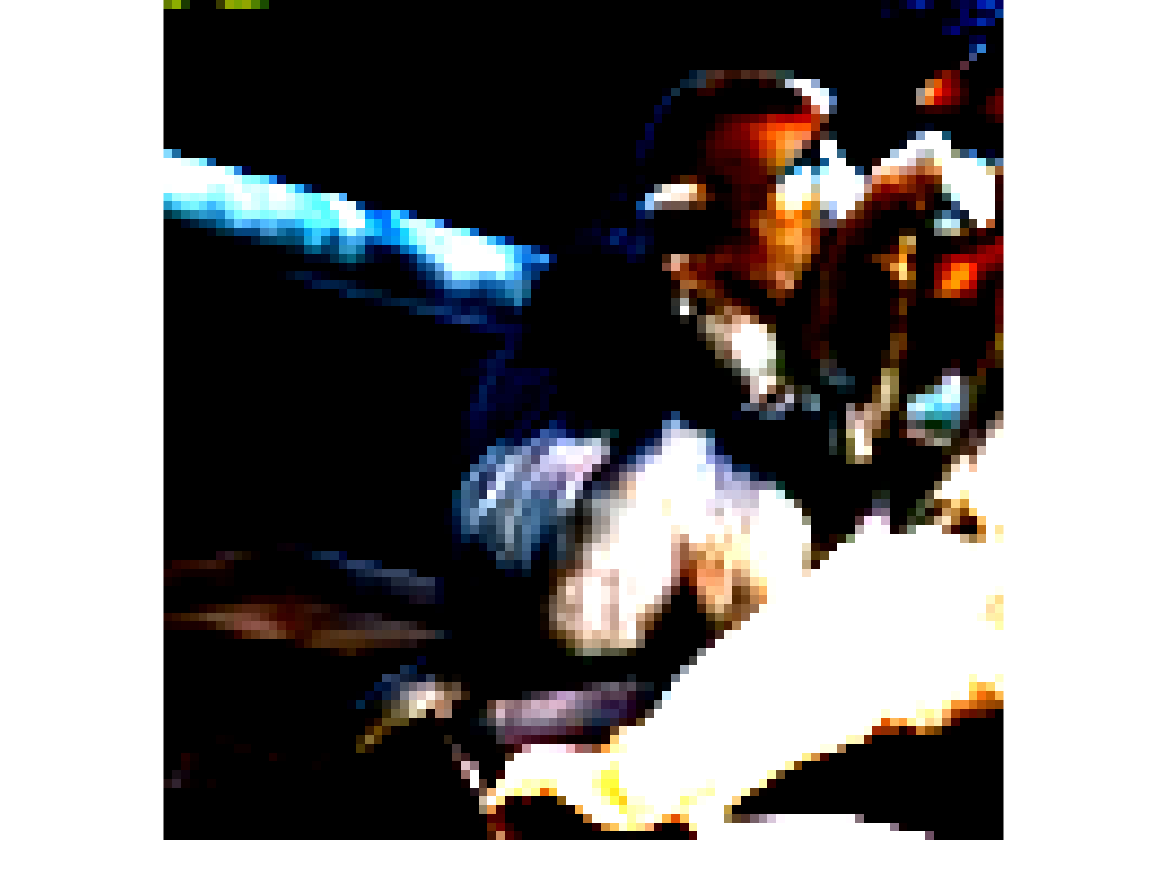
\includegraphics[width=1.8cm]{stl-monkey-1}
			&
			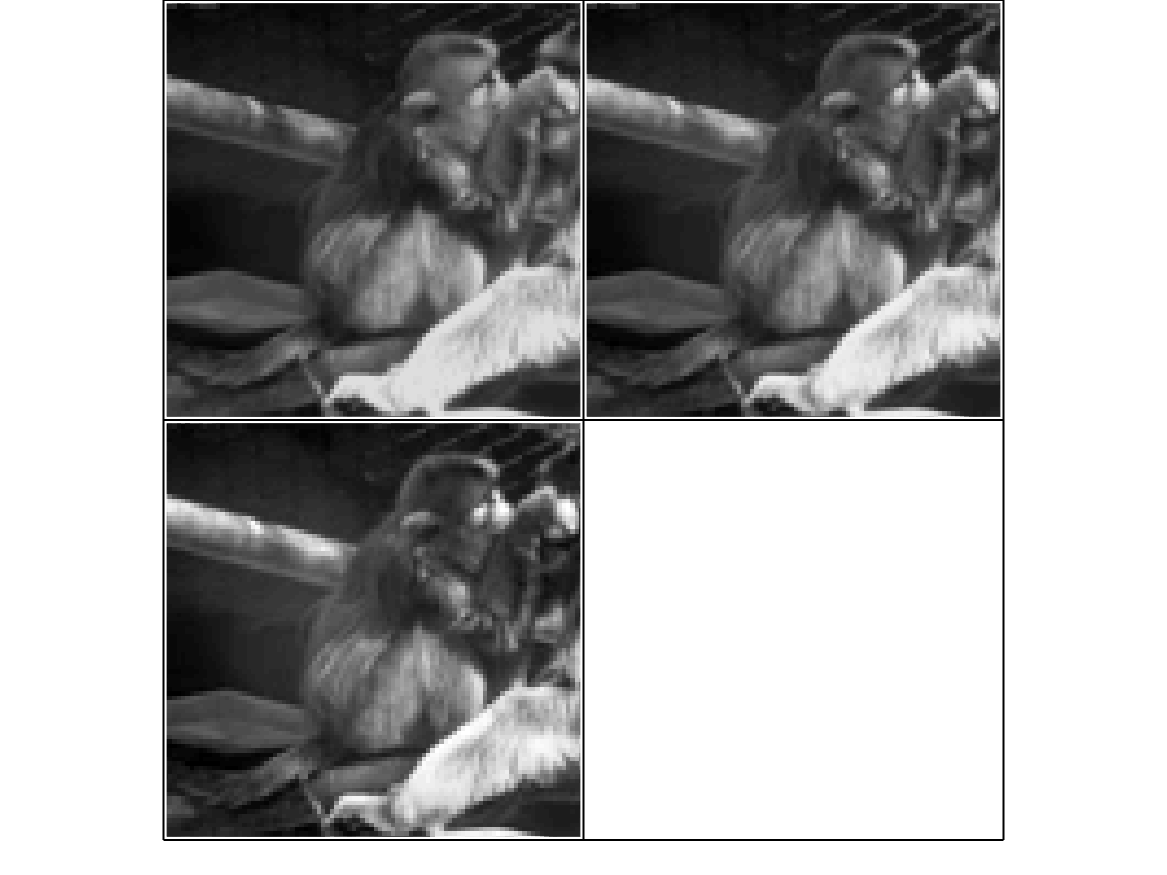
\includegraphics[width=3.6cm]{stl-monkey-2}
			&
			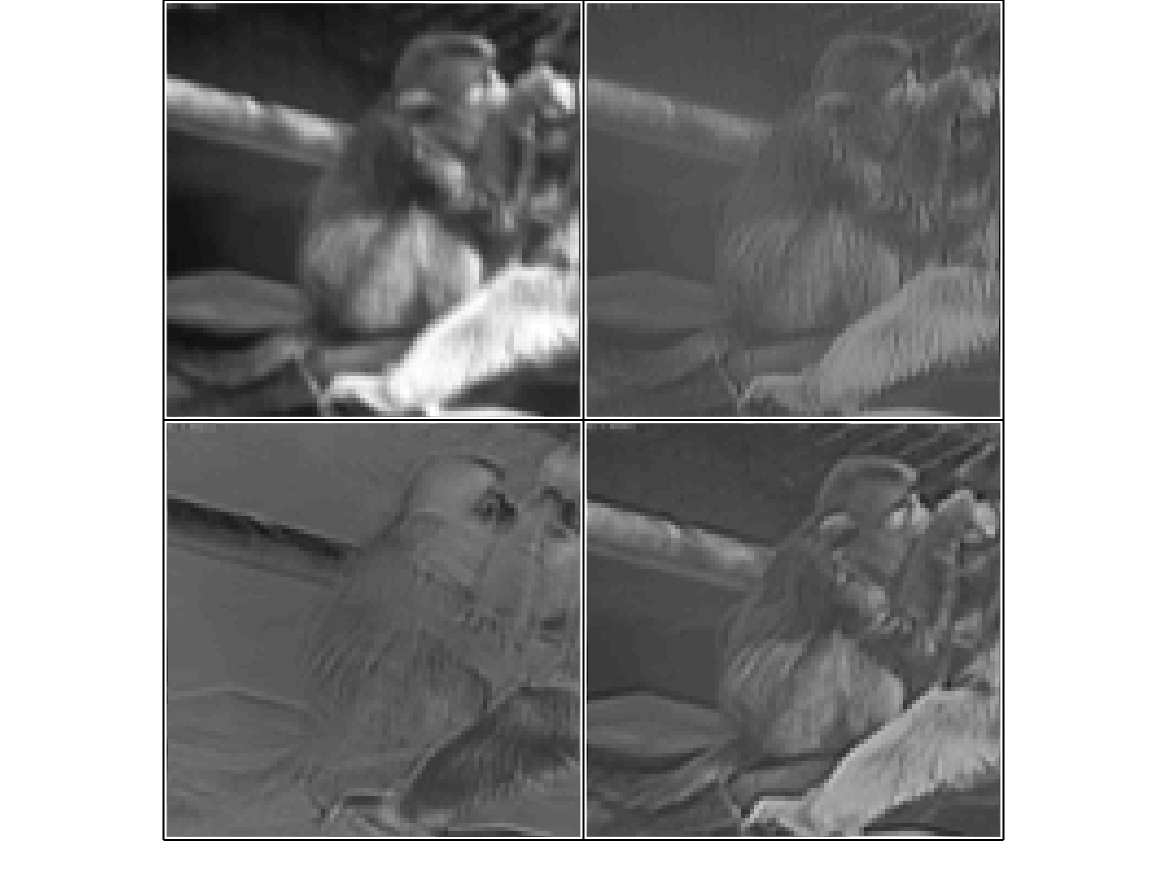
\includegraphics[width=3.6cm]{stl-monkey-3}
		\end{tabular}
	\end{center}
	\pause
	
	Width of CNN can be controlled by number of input and output channels of each layer. Let $\bfy = (\bfy_R, \bfy_G, \bfy_B)$, then we might compute
	$$
		\left(
			\begin{array}{r}
				\bfz_1 \\
				\bfz_2 \\
				\bfz_3 \\
				\bfz_4
			\end{array}
		\right)
		= 
		\left(
		\begin{array}{rrr}
			\bfK^{11}(\bftheta^{11}) &  \bfK^{12}(\bftheta^{12}) & \bfK^{13}(\bftheta^{13})\\
			\bfK^{21}(\bftheta^{21}) &  \bfK^{22}(\bftheta^{22}) & \bfK^{23}(\bftheta^{23})\\
			\bfK^{31}(\bftheta^{31}) &  \bfK^{32}(\bftheta^{32}) & \bfK^{33}(\bftheta^{33})\\
			\bfK^{41}(\bftheta^{41}) &  \bfK^{42}(\bftheta^{42}) & \bfK^{43}(\bftheta^{43})\\
		\end{array}
		\right)
		\left(
			\begin{array}{r}
				\bfy_R \\
				\bfy_G \\
				\bfy_B 
			\end{array}
		\right),
	$$
	where $\bfK^{ij}$ is a 2D convolution operator with stencil $\bftheta^{ij}$
	
\end{frame}

\begin{frame}\frametitle{Outlook: Possible Extensions}
	For now, we just introduced the very basic convolution layer. 
	
	CNNs used in practice also use the following components 
	\begin{itemize}
		\item \emph{pooling:} reduce image resolution (e.g.  average over patches)
		\item \emph{stride:} Example: stride of two reduces image resolution by computing $\bfz$ only at every other pixel. 
	\end{itemize}
	
	\bigskip
	
	Build your own parametric model (ideas for projects)
	\begin{itemize}
		\item $M-$matrix for convolution
		\item cheaper convolution models: separable kernels, doubly symmetric kernels
		\item Wavelet, \ldots
		\item other sparsity patterns
	\end{itemize}
	
\end{frame}

\begin{frame}[allowframebreaks]
	\frametitle{References}
\bibliographystyle{abbrv}
\bibliography{NumDNN}
\end{frame}

\end{document}
